\documentclass{beamer}[10]
\usepackage{pgf}
\usepackage[english]{babel}
\usepackage[utf8]{inputenc}
%\usepackage{beamerthemesplit}
\usepackage{graphics,epsfig, subfigure}
\usepackage{url}
\usepackage{srcltx}
\usepackage{hyperref}

\usepackage{mathrsfs}

\usepackage{amsfonts}

\usepackage{bbm}

\usepackage{amsmath}

\usepackage{amssymb}

\usepackage{amsthm}

\usepackage{blkarray}

\usepackage{dsfont}

\usepackage{enumerate}

\usepackage{graphicx}

\usepackage{centernot}

\usepackage{caption}

\usepackage{braket}

\usepackage{slashed}

\usepackage{pgfplots}

\usepackage{feynmp-auto}

\usepackage{lastpage}

\usepackage{fancyhdr}
\usepackage[square,sort,comma,numbers]{natbib}

\usetikzlibrary{shapes.misc}

\tikzset{cross/.style={cross out, draw=black, minimum size=2*(#1-\pgflinewidth), inner sep=0pt, outer sep=0pt},
	%default radius will be 1pt. 
	cross/.default={2pt}}

\newcommand{\euler}[1]{\text{e}^{#1}}


\newcommand{\Real}{\text{Re}}

%For linespacing=1
\newcommand{\bbra}[2]{\left\langle\begin{matrix}\vspace*{-0.1cm}
		#2\\\vspace*{0.05cm}#1
	\end{matrix}\right\rvert}

\newcommand{\bket}[2]{\left\lvert\begin{matrix}\vspace*{-0.1cm}
		#2\\\vspace*{0.05cm}#1
	\end{matrix}\right\rangle}
\newcommand{\bbraket}[4]{\left\langle\begin{matrix}\vspace*{-0.1cm}
		#2\\ \vspace*{0.05cm}#1
	\end{matrix}\right\vert\left.\begin{matrix}\vspace*{-0.1cm}
	#4\\\vspace*{0.05cm}#3
\end{matrix}\right\rangle}

%\usepackage[all]{xy}


%For linespacing=1.5
%\newcommand{\bbra}[2]{\Big\langle\begin{matrix}\vspace*{-0.35cm}
%		#2\\\vspace*{0.15cm}#1
%	\end{matrix}\Big\rvert}
%
%\newcommand{\bket}[2]{\Big\lvert\begin{matrix}\vspace*{-0.35cm}
%		#2\\\vspace*{0.15cm}#1
%	\end{matrix}\Big\rangle}
%\newcommand{\bbraket}[4]{\Big\langle\begin{matrix}\vspace*{-0.35cm}
%		#2\\ \vspace*{0.15cm}#1
%	\end{matrix}\Big\vert\begin{matrix}\vspace*{-0.35cm}
%	#4\\\vspace*{0.15cm}#3
%\end{matrix}\Big\rangle}

\newcommand\Tstrut{\rule{0pt}{2.6ex}}         % = `top' strut
\newcommand\Bstrut{\rule[-0.9ex]{0pt}{0pt}}   % = `bottom' strut

\renewcommand{\ket}[1]{\left\lvert#1\right\rangle}
\renewcommand{\bra}[1]{\left\langle#1\right\rvert}
\newcommand{\sket}[1]{\left|#1\right]}
\newcommand{\sbra}[1]{\left[#1\right|}
\newcommand{\sbraket}[1]{\left[#1\right]}
\newcommand{\Span}[1]{\text{span}\left(#1\right)}
\newcommand{\MHV}{\text{MHV}}
\newcommand{\PT}{\text{PT}}
\newcommand{\Pf}{\text{Pf}}
\newcommand{\AMHV}{\mathcal{A}^{\MHV}}
\newcommand{\TAMHV}{\tilde{\mathcal{A}}^{\MHV}}
\newcommand{\MMHV}{\mathcal{M}^{\MHV}}
\newcommand{\ANMHV}{\mathcal{A}^{\text{N}\MHV}}
\newcommand{\MNMHV}{\mathcal{M}^{\text{N}\MHV}}
\newcommand{\Pfaff}[1]{\text{Pf}\left(#1\right)}
\newcommand{\rPfaff}[1]{\text{Pf}\ '\left(#1\right)}
\newcommand{\chyline}[2]{\draw[line width=0.5mm] (#1) -- (#2)}
\newcommand{\chydashedline}[2]{\draw[line width=0.5mm, dashed] (#1) -- (#2)}
\newcommand{\chydottedline}[2]{\draw[line width=0.5mm, dotted] (#1) -- (#2)}
\newcommand{\chydoubleline}[2]{\draw [double distance=0.9mm, line width=0.5mm] (#1) -- (#2)}

\newcommand{\chydoubledashedline}[2]{\draw [double distance=0.9mm, line width=0.5mm,dashed] (#1) -- (#2)}

\newcommand{\chytripleline}[2]{\chydoubleline{#1}{#2};\chyline{#1}{#2}
}

\newcommand{\chyquadrupleline}[2]{\draw [double distance=1.6mm, line width=0.5mm] (#1) -- (#2);
	\draw [double distance=0.3mm, line width=0.4mm] (#1) -- (#2)}

\newcommand{\chytripledashedline}[2]{\chydoubledashedline{#1}{#2};\chydashedline{#1}{#2}
}	

\newcommand{\polygonn}[2][]{
	\pgfmathsetmacro{\angle}{360/#2}
	\pgfmathsetmacro{\startangle}{-90-\angle/2}
	\pgfmathsetmacro{\y}{cos(\angle/2)}
	\tikzstyle{vertex}=[circle,fill=black,minimum size=7pt,text width = 7pt,inner sep=0pt]
	\foreach \i in {1,2,...,#2} {
		\pgfmathsetmacro{\x}{\startangle - \angle*\i}
		\node[vertex] (p\i) at (\x+\angle:1cm) [label={[label distance= -0.1mm]\x+\angle:$ \i $}] {};
	}
	
	
}
\newcommand{\polygonnn}[2][]{
	\pgfmathsetmacro{\angle}{360/#2}
	\pgfmathsetmacro{\startangle}{-90-\angle/2}
	\pgfmathsetmacro{\y}{cos(\angle/2)}
	\tikzstyle{vertex}=[circle,fill=black,minimum size=7pt,text width = 7pt,inner sep=0pt]
	\foreach \i in {1,2,...,#2} {
		\pgfmathsetmacro{\x}{\startangle - \angle*\i}
		\node[vertex,scale=0.1] (\i) at (\x+\angle:1cm) {};
	}
}
\newenvironment{polygon}[1][]
{	\def\myenvargumentII{#1} 
	\polygonnn{#1}}
{\polygonn{\myenvargumentII}
}

\newenvironment{chy}[1][]
{
	\begin{gathered}
		\begin{tikzpicture}[scale=0.65]
			\begin{polygon}[#1]
			}
			{
			\end{polygon}
		\end{tikzpicture}
	\end{gathered}
}



% TikZ til at lave figurer - for de avancerede
\usepackage{tikz}
% Div. pakker (muligt at ikke alle er i brug)
\usetikzlibrary{decorations.pathmorphing}
\usetikzlibrary{arrows.meta}
\usetikzlibrary{arrows}
\usetikzlibrary{decorations.pathreplacing,decorations.markings}
\usetikzlibrary{patterns}
\usetikzlibrary{fadings}
\usetikzlibrary{calc}
\usetikzlibrary{tikzmark,fit,shapes.geometric}

\definecolor{kugreen}{RGB}{79,112,148}
\definecolor{kugreenlys}{RGB}{255,242,204}
\definecolor{kugreenlyslys}{RGB}{173,190,177}
\definecolor{kugreenlyslyslys}{RGB}{214,223,216}
\setbeamercovered{transparent}
\mode<presentation>
%\usetheme[numbers,totalnumber,compress,sidebarshades]{PaloAlto}
\setbeamertemplate{footline}[frame number]
  \usecolortheme[named=kugreen]{structure}
  \useinnertheme{circles}
  \usefonttheme[onlymath]{serif}
  \setbeamercovered{transparent}
  \setbeamertemplate{blocks}[rounded][shadow=false]
  \setbeamercolor{block title}{bg=kugreen,fg=black}
	\setbeamercolor{block body}{bg=kugreenlys,fg=black}
\logo{
\includegraphics[width=1.4cm]{kuscience-logo}}
%\useoutertheme{infolines} 
\title{Riemann Surfaces}
\subtitle{An introduction}
\author{Taro Valentin Brown}
\institute{University of California, Davis}
\date{May 26, 2021.}
\setbeamercovered{invisible}

\begin{document}
\frame{\titlepage \vspace{-0.5cm}
}

\frame
{
\frametitle{Overview}
\linespread{1.5}
\tableofcontents%[pausesection]
}
\section{Idea of Riemann Surfaces}
\begin{frame}
	\frametitle{Recap of complex analysis so far}
	\begin{block}{Functions of one complex variable}
	Take some open set $U$ in the complex plane and a function $f$ which takes complex variables $z$ and maps them to $\omega=f(z)$ in the open domain $V$
	\end{block}
\begin{figure}
	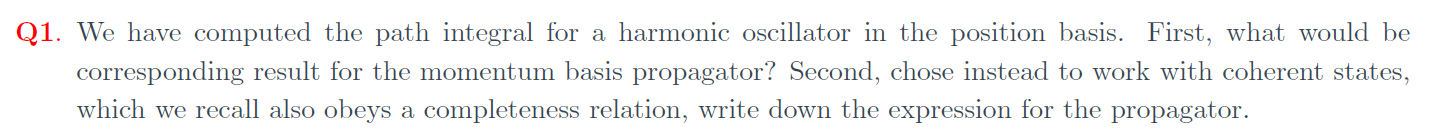
\includegraphics[width=8cm]{1.PNG}
\end{figure}
\end{frame}

\begin{frame}
	\frametitle{Recap of complex analysis so far}
	\begin{block}{Functions of one complex variable}
	Requiring $f$ to be holomorphic in a neighborhood around $z_0$ put great constraints on our functions, i.e. Cauchy Riemann conditions (among others) with $\omega=u+iv$, $z=x+iy$
	\begin{equation}
		\begin{aligned}
			\partial_x u= \partial_y v,~~~~\partial_x v= -\partial_y u
		\end{aligned}
	\end{equation}
	\end{block}
\end{frame}

\begin{frame}
	\frametitle{Some definitions}
	\begin{block}{Some definitions}
	\begin{itemize}
		\item \textbf{Isomorphism}: Structure-preserving mapping between two structures of the same type that can be reversed by an inverse mapping.
		\item \textbf{Homeomorphism}: Isomorphism in the category of topological spaces. I.e. they are the mappings that preserve all the topological properties of a given space
		\item  \text{Injective holomorphic map} is a holomorphic isomorphism
	\end{itemize}
Given a holomorphic injective map from an open set $U$ to $\mathds{C}$
\begin{equation}
	\begin{aligned}
		f:U \to \mathds{C}
	\end{aligned}
\end{equation}
then $f(U)$ is open, and the inverse map is also holomorphic.
	\end{block}
\end{frame}

\begin{frame}
	\frametitle{Complex analysis on surfaces}
	\begin{block}{Complex analysis on surface}
		\begin{itemize}
			\item Take a known surface that we can visualize.
			\item Pick some point $x_0$ on the surface on some disc-like domain $\mathcal{D}$.
			\item Introduce function $f:\mathcal{D}\to \mathds{C}$ that takes on complex values on $\mathcal{D}$.
			\item Extend definition of holomorphic function at $x_0$ so that we can use tools of complex analysis on the surface.
		\end{itemize}
	\end{block}
\begin{figure}
	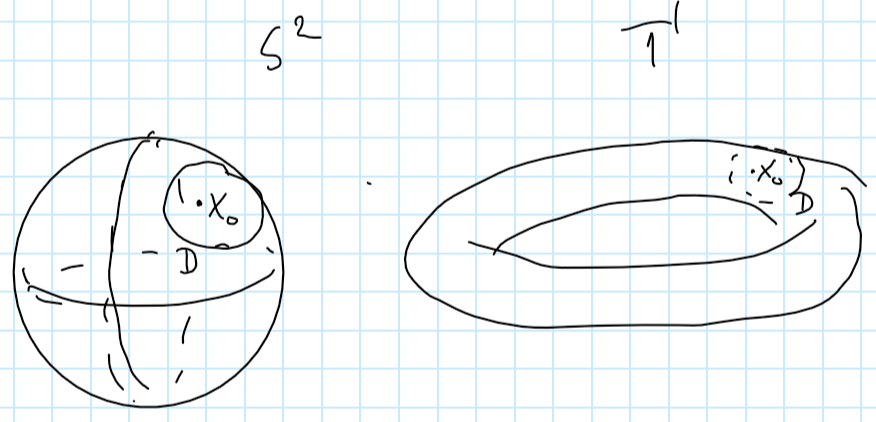
\includegraphics[width=10cm]{2.PNG}
\end{figure}
\end{frame}

\begin{frame}
	\frametitle{Pick a simple surface}
	\begin{block}{Pick a simple surface}
			Do this by identifying $\mathcal{D}$ with an open subset, say
			\begin{equation}
				\begin{aligned}
					\Delta = \{z\in \mathds{C}~\big|~|z|=1\}
				\end{aligned}
			\end{equation}
		by choosing a homeomorphism 
		\begin{equation}
			\begin{aligned}
				\phi:\mathcal{D}\to \Delta \subset \mathds{C}
			\end{aligned}
		\end{equation}
	Hence we now have a map from the unit disc on the surface to the complex plane
\begin{figure}\vspace*{-0.3cm}
	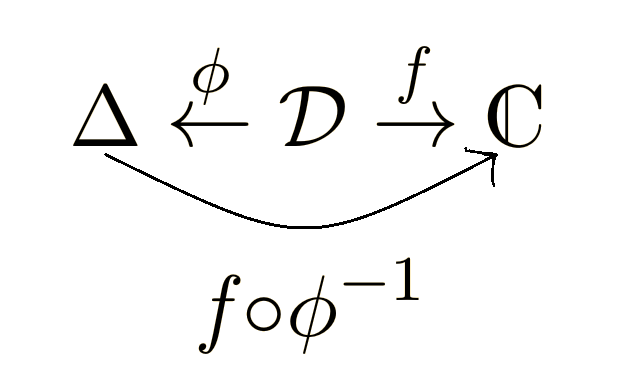
\includegraphics[width=2.7cm]{3}
\end{figure}
and require that $f\circ \phi^{-1}$ is holomorphic at the point.
	\end{block}
\end{frame}

\begin{frame}
	\frametitle{Holomorphic requirement}
	\begin{block}{Holomorphic requirement}
	So: we get a function from the disc in the complex plane to the complex numbers.\\
	\vspace*{0.5cm}
	Here it is it is easy to see when it is holomorphic at $x_0$.\\
		\vspace*{0.5cm}
	 $f$ is holomorphic on all of $\mathcal{D}$ if $f\circ \phi^{-1}$ is holomorphic on $\Delta$.\\
	\end{block}
\end{frame}

\begin{frame}
	\frametitle{Complex coordinate chart}
	\begin{block}{Complex coordinate chart}
	The pair $(\mathcal{D},\phi)$ is called a \textit{complex coordinate chart}\\
	\vspace*{0.5cm}
	It allows us to do complex analysis on the disc\\
	\vspace*{0.5cm}
	In this example $z=\phi(x)$, $x\in X$ provides us with a new symbol in a continuously isomorphic way.\\
	\vspace*{0.5cm}
	The resulting function is a function of one complex variable on an open subset on the complex plane, where we can do complex analysis.
	\end{block}
\end{frame}

\begin{frame}
	\frametitle{Extending to other surfaces}
	\begin{block}{Extending to other surfaces}
		\vspace*{0.5cm}
		We could have taken any open set, not just a disc-like neighborhood.\\
		\vspace*{0.5cm}
		Would have to choose a different homeomorphism to an open set on the complex plane.
	\end{block}
\end{frame}

\begin{frame}
	\frametitle{Extending to other surfaces}
	\begin{block}{Extending to other surfaces}
		More generally: a complex coordinate chart is a pair
		\begin{equation}
			\begin{aligned}
				(\mathcal{U},\phi)
			\end{aligned}
		\end{equation}
	where $\mathcal{U}$ is an open subset of $X$ and $\phi:\mathcal{U}\to \mathcal{V}$ is a homemorphism onto an open subset $\mathcal{V}$ of $\mathds{C}$.\\
	\vspace*{0.5cm} If we we have a function $f$ on $\mathcal{D}$ that takes complex values, $f$ is holomorphic if $f\circ \phi^{-1}$ is holomorphic.
	\end{block}
\begin{figure}
	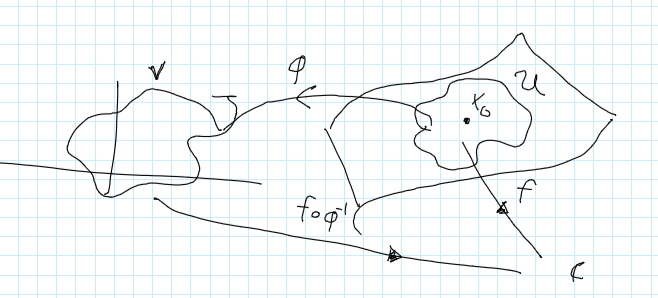
\includegraphics[width=7cm]{4}
\end{figure}
\end{frame}

\begin{frame}
	\frametitle{Naïve preliminary definition of Riemann Surface}
	\begin{block}{Riemann surface}
	A surface $X$ covered by a collection of charts that span of all of $X$
	\begin{equation}
		\begin{aligned}
			\{(\mathcal{U}_\alpha,\phi_\alpha)~\big|~\alpha\in I\}
		\end{aligned}
	\end{equation}
	\end{block}
\end{frame} 

\begin{frame}
	\frametitle{Naïve preliminary definition of Riemann Surface}
	\begin{block}{Problem since charts can in principle intersect}
		Consider e.g. 
		\begin{equation}
			\begin{aligned}
				f:\mathcal{U}_{\alpha_1}\cap \mathcal{U}_{\alpha_2}\to \mathds{C}
			\end{aligned}
		\end{equation}
	so we have two charts $(\mathcal{U}_{\alpha_1},\phi_{\alpha_1})$ and $(\mathcal{U}_{\alpha_2},\phi_{\alpha_2})$. To be a Riemann surface, both charts should be holomorphic in the domain.
	\end{block}
\begin{figure}
	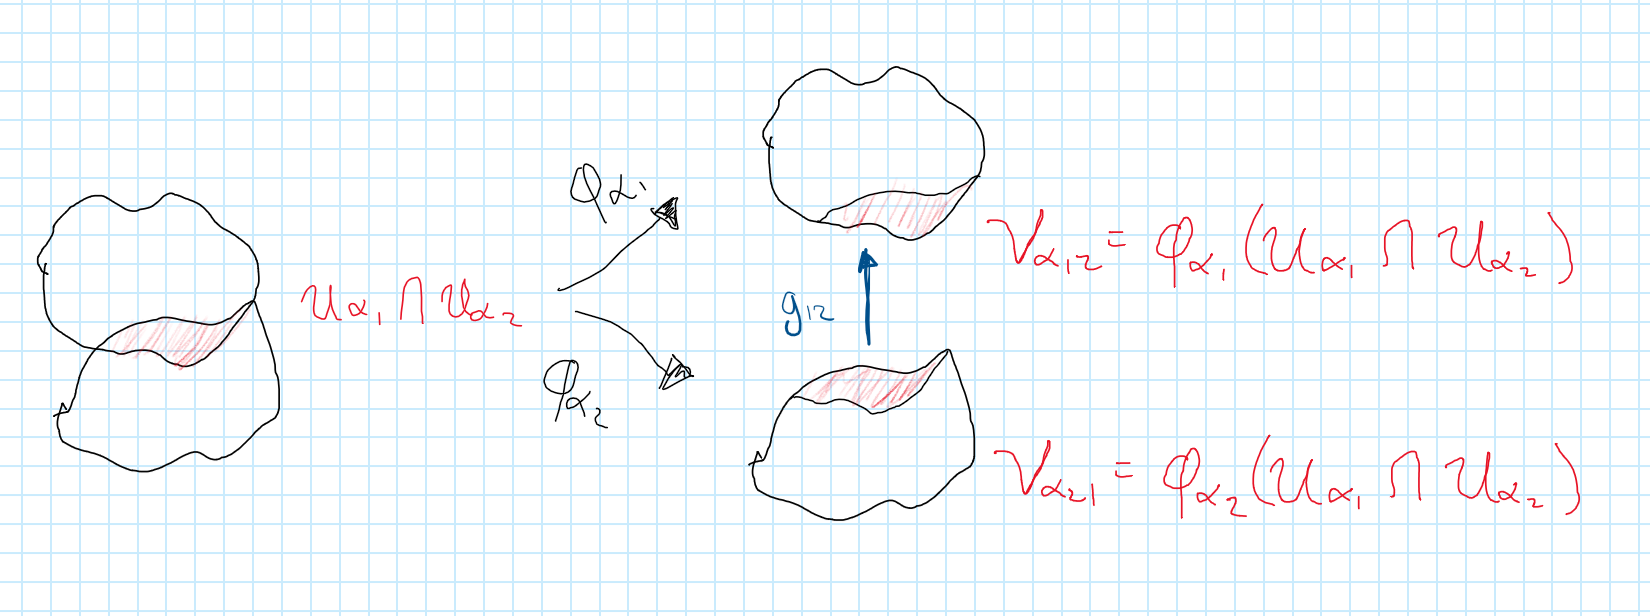
\includegraphics[width=10cm]{5}
\end{figure}
\end{frame} 


\begin{frame}
	\frametitle{Naïve preliminary definition of Riemann Surface}
	\begin{block}{Problem since charts can in principle intersect}
	We then require the transition function $g_{12}$ between $\mathcal{V}_{\alpha_{12}}$ and $\mathcal{V}_{\alpha_{21}}$ to be holomorphic
	\begin{equation}
		\begin{aligned}
			g_{12}=\phi_{\alpha_1}\big|_{\mathcal{U}_{\alpha_1}\cap \mathcal{U}_{\alpha_2}}\circ \phi_{\alpha_2}^{-1}\big|_{\mathcal{U}_{\alpha_1}\cap \mathcal{U}_{\alpha_2}}
		\end{aligned}
	\end{equation}
	since this condition leads to (ignoring subscripts)
	\begin{equation}
		\begin{aligned}
			f\circ \phi_{\alpha_1}^{-1}\circ g_{12}=f\circ \phi_{\alpha_2}^{-1}
		\end{aligned}
	\end{equation}
$g_{12}$ is holomorphic isomorphism from the holomorphic requirement (i.e. it has an inverse $g_{21}$)\\ This implies that
	$\phi^{-1}_{\alpha_1}$ and $\phi^{-1}_{\alpha_2}$ have to both be holomorphic. \\
	It is exactly what we wanted!
	\end{block}
\end{frame} 

\begin{frame}
	\frametitle{Definition of Riemann Surface}
	\begin{block}{Summary}
	\begin{itemize}
		\item We require that transition functions are holomorphic for $\mathcal{U}_{\alpha_1}\cap \mathcal{U}_{\alpha_2}\neq \emptyset$
		\item This gives us a collection of charts that are \textit{compatible}
		\item Such a collection that covers all of $X$ is known as a complex \textit{Atlas}
		\item A surface $X$ is a Riemann surface if there exists such an atlas.
	\end{itemize}
	\end{block}
\end{frame} 
\section{Riemann surface definition and examples}
\begin{frame}
	\frametitle{Examples of Riemann Surfaces}
	\begin{block}{Example I: $X=\mathds{R}^2$}
		We only need one chart
		\begin{equation}
			\begin{aligned}
				X=\{(\mathds{R}^2,\phi)\}
			\end{aligned}
		\end{equation}
		with
		\begin{equation}
			\begin{aligned}
				\phi: \mathds{R}^2\to \mathds{C}
			\end{aligned}
		\end{equation}
	I.e. $(x,y)\to x+iy$. The holomorphic functions on $X$ are the holomorphic functions on $\mathds{C}$.
	\end{block}
\begin{figure}
	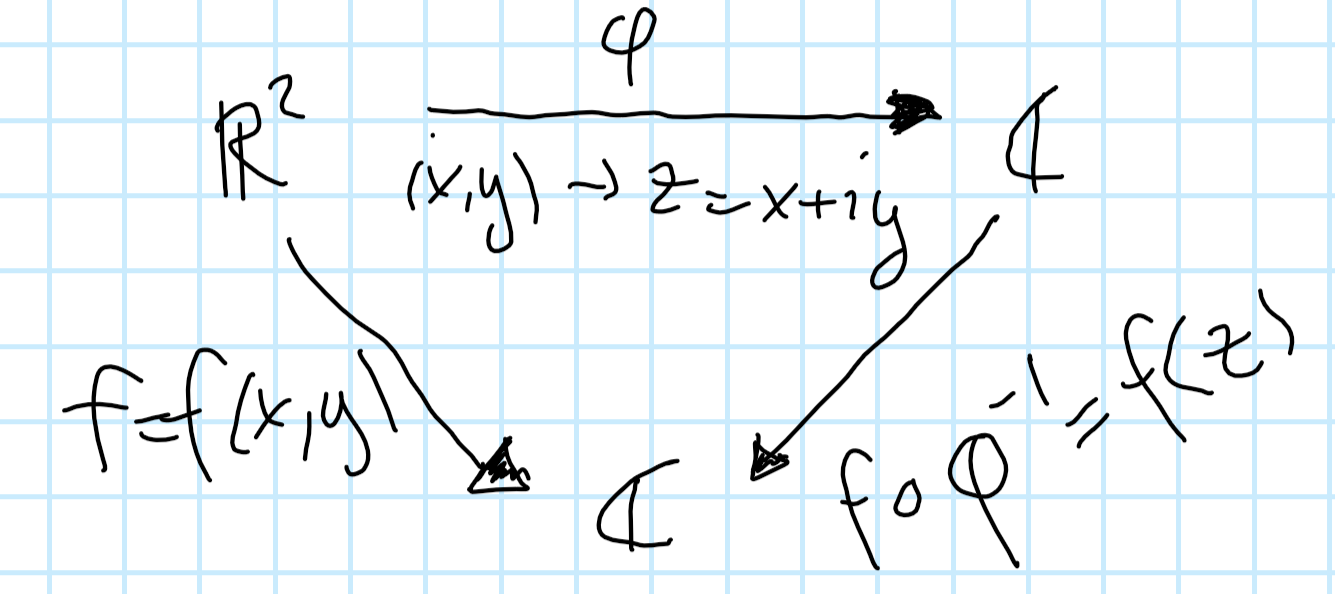
\includegraphics[width=6cm]{6}
\end{figure}
\end{frame} 

\begin{frame}
	\frametitle{Examples of Riemann Surfaces}
	\begin{block}{Example I: $X=\mathds{R}^2$}
	We could also have taken a difference chart $\phi:\mathds{R}^2\to \mathds{C}$ with 
		\begin{equation}
			\begin{aligned}
			\phi:(x,y)&\mapsto \frac{z}{1+|z|}=\frac{x}{1+\sqrt{x^2+y^2}}+i\frac{y}{1+\sqrt{x^2+y^2}}\\
			\phi^{-1}:z&\mapsto \frac{z}{1-|z|}=\left(\frac{x}{1-\sqrt{x^2+y^2}},\frac{y}{1-\sqrt{x^2+y^2}}\right)
			\end{aligned}
		\end{equation}
	(I.e.) mapping $\mathds{C}$ onto $\Delta$. This is a homeomorphism. This is not the same Riemann surface!
	\end{block}
\end{frame}

\begin{frame}
	\frametitle{Examples of Riemann Surfaces}
	\begin{block}{Example I: $X=\mathds{R}^2$}
	For $f$ to be holomorphic, $f\circ \phi^{-1}$ has to also be. 
	\begin{equation}
		\begin{aligned}
			f\circ \phi^{-1}(z)=f\left(\frac{z}{1-|z|}\right)=f\left(\frac{x}{1-\sqrt{x^2+y^2}},\frac{y}{1-\sqrt{x^2+y^2}}\right)
		\end{aligned}
	\end{equation}
Not holomorphic for the natural identification $f(x,y)\to x+iy=z$
\begin{equation}
	\begin{aligned}
		f\left(\frac{z}{1-|z|}\right)=\frac{z}{1-|z|}
	\end{aligned}
\end{equation}
Completely different structure! It is the Riemann surface structure on the unit disc.\\
\vspace*{0.2cm} Riemann mapping theorem: unit disc is not equal to complex plane. 
\end{block}
	\end{frame}

\begin{frame}
	\frametitle{Examples of Riemann Surfaces}
	\begin{block}{Example: $X=S^2$}
		Take the two-dimensional sphere.	
	\end{block}
	\begin{figure}\vspace*{-0.7cm}\hspace*{-0.7cm}
		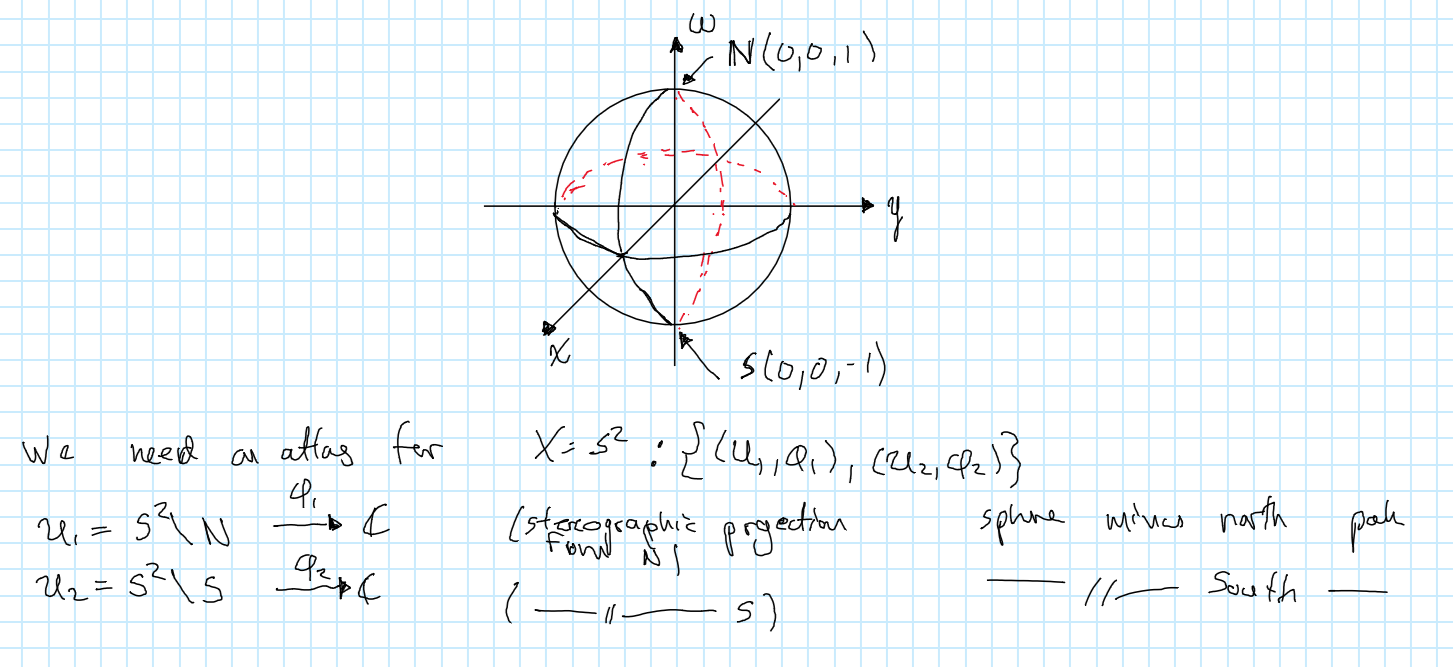
\includegraphics[width=12cm]{7}
	\end{figure}
\end{frame}

\begin{frame}
	\frametitle{Examples of Riemann Surfaces}
	\begin{block}{Example: $X=S^2$}
	Stereographic projection works in the following way
	\end{block}
	\begin{figure}
		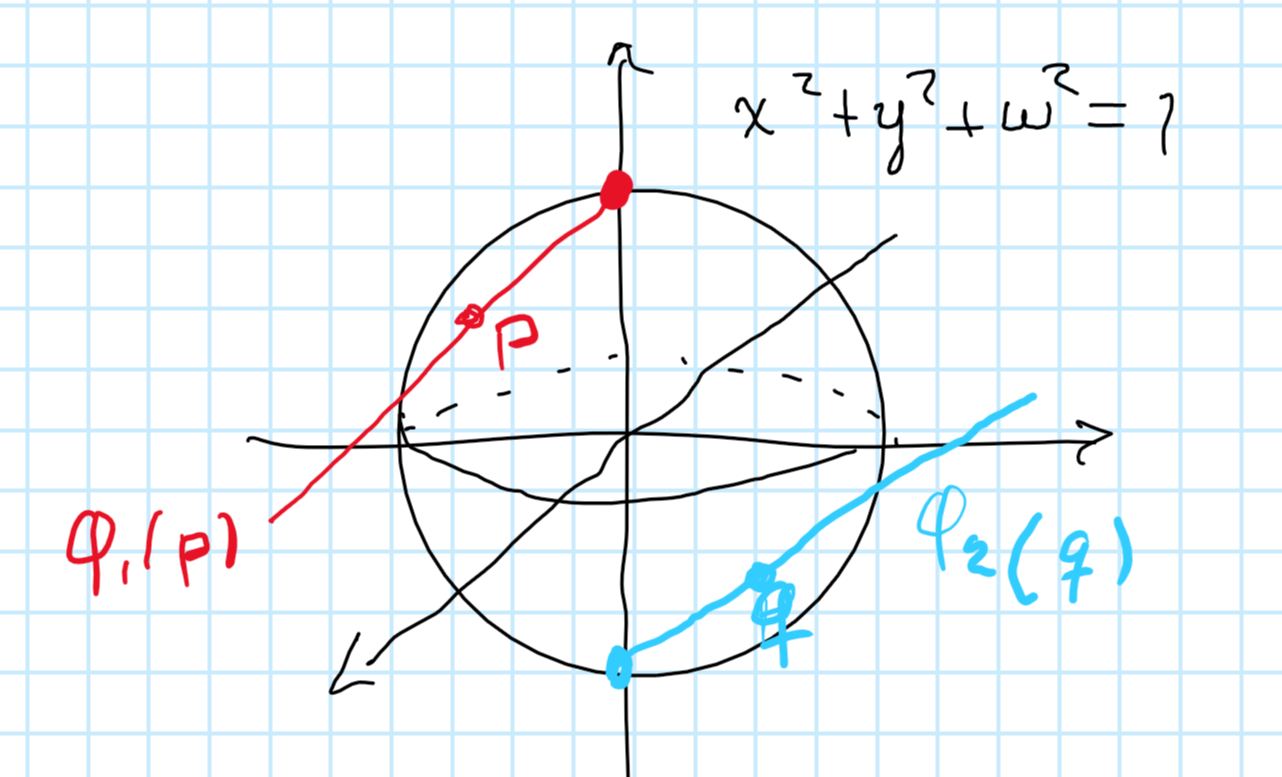
\includegraphics[width=6cm]{8}
	\end{figure}
	$\phi_1(p)=$ point of intersection of north pole with $xy$-plane\\
	$\phi_2(p)=$ point of intersection of south pole with $xy$-plane
\end{frame}

\begin{frame}
	\frametitle{Examples of Riemann Surfaces}
	\begin{block}{Check for compatiblity}
	\begin{equation}
		\begin{aligned}
			\mathcal{U}_{1}\cap \mathcal{U}_{2}&=S^2\backslash\{N,S\}\\
			\phi_1(\mathcal{U}_{1}\cap \mathcal{U}_{2})&=\mathds{C}\backslash\{0\}\\
			\phi_2(\mathcal{U}_{1}\cap \mathcal{U}_{2})&=\mathds{C}\backslash\{0\}
		\end{aligned}
	\end{equation}
	The transition function from $\mathds{C}\backslash\{0\}\to \mathds{C}\backslash\{0\}$ is $z\to \frac{1}{z}$, which is holomorphic. This Riemann surface structure is the Riemann Sphere\\
	Are there any more atlas?
	\end{block}
\end{frame}

\begin{frame}
	\frametitle{Examples of Riemann Surfaces}
	\begin{block}{Uniformization Theorem}
	Every simply connected Riemann surface is conformally equivalent to one of three Riemann surfaces: the open unit disk $\Delta$, the complex plane $\mathds{C}$, or the Riemann sphere $\mathds{C}\cup \infty$.\\
	\vspace*{0.3cm}
	\textit{Simply connected}: I.e. an object which consists of one piece and does not have any holes that pass all the way through it.
	\end{block}
\end{frame}

\begin{frame}
	\frametitle{Examples of Riemann Surfaces}
	\begin{block}{Automorphisms}
		Final note before we look at applications.\\
		 Automorphisms of the Riemann sphere are Möbius transformations
		 \begin{equation}
		 	\begin{aligned}
		 		z\to \frac{az+b}{cz+d},~~~~ad-bc=1
		 	\end{aligned}
		 \end{equation}
	\end{block}
\end{frame}


\section{Applications}
\begin{frame}
	\frametitle{Applications}
	\begin{block}{QFT scattering}
		Overlap between two asymptotic states
		\begin{equation}\label{ScatteringMatrix}
		\braket{f|i}=(2\pi)^D\delta^D\left(\sum_ik_i\right)(\mathds{1}_{fi}+iT_{fi}),
		\end{equation}
		Scattering cross section proportional to $|T_{fi}|^2$.
		
		We refer to $ T_{fi} $ as the scattering amplitude and denote it by $ \mathcal{A}(...) $ where $ (...) $ is the scattering data.
	\end{block}
\end{frame}


\begin{frame}
	\frametitle{The Scattering Equations}
	\begin{block}{Scattering equations and amplitudes}
		The \emph{scattering equations} live on the Riemann sphere through $z_i$ and are given by
		\begin{equation}
		\mathcal{S}_i=\sum_{j\neq i}\frac{s_{ij}}{z_i-z_j}=0,\quad i\in\{1,2,..,n\}.	\label{ScatteringEquations}
		\end{equation}
		One can obtain amplitudes of various theories from the formula
		\begin{equation}
		\mathcal{A}_n(1,...,n)=\int d\Omega_{\text{CHY}} \mathcal{I}(z_i,k_i,\epsilon_i,...), \label{CHYformula1}
		\end{equation}
		with $ d\Omega_{\text{CHY}}=\frac{d^nz}{\text{Vol}(\text{SL}(2,\mathbb{C}))}\prod_{i}'\delta(\mathcal{S}_i) $.
	\end{block}
\end{frame}

\begin{frame}
	\frametitle{Complex analysis tools}
	\begin{block}{Scattering equations and amplitudes}
		Since the space is the Riemann sphere, one can use tools of complex analysis. Remember
		\begin{equation}
			\begin{aligned}
				f(a)&=\frac{1}{2\pi i}\oint \text{d}z\,\frac{f(z)}{z-a}
			\end{aligned}
		\end{equation}
	Reformulate the delta-functions $\to$ use complex analysis. \\
	\vspace*{0.5cm}
	From the global residue theorem one can obtain diagrammatic rules to calculate amplitudes.
	\end{block}
\end{frame}


\begin{frame}
	\frametitle{Integration rules}
	\begin{block}{Graphic representation of Möbius invariant integrands}
		We represent the integrands by four-regular graphs. Every factor of $ z_{ij}^{-1} $ is a line between vertices $ i $ and $ j $ and every factor $ z_{ij} $ is a dashed line. 
		\begin{equation}
			A_n^{\varphi^3}(1,2,3,\dots,n)=\int\text{d}\Omega_{\text{CHY}}\frac{1}{z_{12}^2z_{23}^2\cdots z_{n1}^2}.
		\end{equation}
	The integrand is 
	\begin{equation} \label{eq:4pt-ex}
	\mathcal{I}(z)=\frac{1}{z_{12}^2z_{23}^2z_{34}^2z_{41}^2}\to
	\begin{chy}[4]
		\chydoubleline{1}{2};
		\chydoubleline{2}{3};
		\chydoubleline{3}{4};
		\chydoubleline{4}{1};
	\end{chy}.
\end{equation}
	\end{block}
\end{frame}

\begin{frame}
	\frametitle{Integration rules}
	\begin{block}{Graphic representation of Möbius invariant integrands}
	Using simple derived rules
	\begin{equation} \label{eq:4pt-expr}
		\begin{chy}[4]
			\chydoubleline{1}{2};
			\chydoubleline{2}{3};
			\chydoubleline{3}{4};
			\chydoubleline{4}{1};
		\end{chy}
		\to
		-\frac{1}{s_{12}}-\frac{1}{s_{14}},
	\end{equation}
	We get the final amplitude to be
	\begin{equation}
		A_4^{\varphi^3}(1,2,3,4)=-\frac{1}{s_{12}}-\frac{1}{s_{14}}.
	\end{equation}
It only took 1 diagram!
	\end{block}
\end{frame}

\section{Conclusion}
\begin{frame}
	\frametitle{Summary}
	\begin{block}{}
		\begin{itemize}
			\item Started with a real surface $X$ on which we wanted to do complex analysis
			\item This was achieved by using complex charts $\{(\mathcal{U}_i,\phi_i)\big|i\in I\}$ such that $\mathcal{U}_i$ covers all of $X$
			\item We checked that $f$ was holomorphic by using $f\circ \phi^{-1}$
			\item Compatible charts (atlas) were introduced to make sure the functions were holomorphic even if charts overlapped.
			\item We analyzed different Riemann structures and introduced the uniformization theorem.
			\item Finally an application in scattering amplitudes was reviewed.
		\end{itemize}
	\end{block}
\end{frame}

\begin{frame}
	\centering
	\Large Thank you for your attention.\\
\end{frame}		
\end{document}
